\documentclass[a4paper, 12pt, slovene]{article}
\usepackage[slovene]{babel}
\usepackage[utf8]{inputenc}
\usepackage{lmodern}
\usepackage[T1]{fontenc}
\usepackage{graphicx}
\usepackage{caption}
\captionsetup{font=footnotesize}
\usepackage{fullpage}
\usepackage{enumitem}
\usepackage{array}
\usepackage{wrapfig}
\usepackage{multirow}
\usepackage{tabularx}
\usepackage{amsmath}
\usepackage{amssymb}
\usepackage{subcaption}
\newcommand*\diff{\mathop{}\!\mathrm{d}}
\newcommand*\Diff[1]{\mathop{}\!\mathrm{d^#1}}
\newcommand*\difft{\mathop{}\!\ddot{ }}
\usepackage{float}
\usepackage{mathrsfs}
\usepackage{fancyvrb}
\usepackage{hyperref}
\usepackage{xurl}
\usepackage{breqn}
\numberwithin{equation}{section}

\newcommand{\Ai}{\mathrm{Ai}}
\newcommand{\Bi}{\mathrm{Bi}}

\renewcommand{\Re}{\mathop{\rm Re}\nolimits}
\renewcommand{\Im}{\mathop{\rm Im}\nolimits}
\newcommand{\Tr}{\mathop{\rm Tr}\nolimits}
\newcommand{\diag}{\mathop{\rm diag}\nolimits}
\newcommand{\dd}{\,\mathrm{d}}
\newcommand{\ddd}{\mathrm{d}}
\newcommand{\ii}{\mathrm{i}}
\newcommand{\lag}{\mathcal{L}\!}
\newcommand{\ham}{\mathcal{H}\!}
\newcommand{\four}[1]{\mathcal{F}\!\left(#1\right)}
\newcommand{\bigO}[1]{\mathcal{O}\!\left(#1\right)}
\newcommand{\sh}{\mathop{\rm sinh}\nolimits}
\newcommand{\ch}{\mathop{\rm cosh}\nolimits}
\renewcommand{\th}{\mathop{\rm tanh}\nolimits}
\newcommand{\erf}{\mathop{\rm erf}\nolimits}
\newcommand{\erfc}{\mathop{\rm erfc}\nolimits}
\newcommand{\sinc}{\mathop{\rm sinc}\nolimits}
\newcommand{\rect}{\mathop{\rm rect}\nolimits}
\newcommand{\ee}[1]{\cdot 10^{#1}}
\newcommand{\inv}[1]{\left(#1\right)^{-1}}
\newcommand{\invf}[1]{\frac{1}{#1}}
\newcommand{\sqr}[1]{\left(#1\right)^2}
\newcommand{\half}{\frac{1}{2}}
\newcommand{\thalf}{\tfrac{1}{2}}
\newcommand{\pd}{\partial}
\newcommand{\Dd}[3][{}]{\frac{\ddd^{#1} #2}{\ddd #3^{#1}}}
\newcommand{\Pd}[3][{}]{\frac{\pd^{#1} #2}{\pd #3^{#1}}}
\newcommand{\avg}[1]{\left\langle#1\right\rangle} 
\newcommand{\norm}[1]{\left\Vert #1 \right\Vert}
\newcommand{\braket}[2]{\left\langle #1 \vert#2 \right\rangle}
\newcommand{\obraket}[3]{\left\langle #1 \vert #2 \vert #3 \right \rangle}
\newcommand{\hex}[1]{\texttt{0x#1}}

\renewcommand{\iint}{\mathop{\int\mkern-13mu\int}}
\renewcommand{\iiint}{\mathop{\int\mkern-13mu\int\mkern-13mu\int}}
\newcommand{\oiint}{\mathop{{\int\mkern-15mu\int}\mkern-21mu\raisebox{0.3ex}{$\bigcirc$}}}

\newcommand{\wunderbrace}[2]{\vphantom{#1}\smash{\underbrace{#1}_{#2}}}

\renewcommand{\vec}[1]{\overset{\smash{\hbox{\raise -0.42ex\hbox{$\scriptscriptstyle\rightharpoonup$}}}}{#1}}
\newcommand{\bec}[1]{\mathbf{#1}}

\newcommand{\bi}[1]{\hbox{\boldmath{$#1$}}}
\newcommand{\bm}[1]{\hbox{\underline{$#1$}}}  

\newcommand{\nap}{\nabla_{\perp}}  

\catcode`_=12
\begingroup\lccode`~=`_\lowercase{\endgroup\let~\sb}
\mathcode`_="8000


\begin{document}

\begin{titlepage}
\title{\textsc{Linearno Programiranje} \\[1ex] \large Druga naloga pri predmetu Modelska analiza 1}
\author{Gašper Lotrič \\ 28191019}
\date{oktober 2022}

\maketitle
\end{titlepage}

\tableofcontents
\pagebreak


\section{Naloga}
Med tipične primere, ki jih lahko učinkovito rešimo z metodami linearnega programiranja, sodi sestavljanje diet za hujšanje, zdravljenje ali športne aktivnosti. Za dani nabor živil določamo njihove količine, pri čemer moramo zadostiti različnim omejitvam. Med drugim moramo zagotoviti priporočene dnevne odmerke mineralov, vitaminov in hranilnih snovi, omejiti pri vnos maščob, ogljikovih hidratov ter telesu škodljivih snovi, hkrati pa zagotoviti, da energijska vrednost ustreza zahtevam posameznika. Vnos vsake izmed hranilnih snovi je linearna funkcija količin živil in je natanko določena z njihovo
sestavo. Od vrste diete pa je odvisno, katere parametre omejimo in katere minimiziramo.
\begin{enumerate}
\item Minimiziraj količino kalorij, če je priporočen minimalni dnevni vnos 70 g maščob, 310 g ogljikovih hidratov, 50 g proteinov, 1000 mg kalcija ter 18 mg železa. Dnevni obroki naj količinsko ne presežejo dveh kilogramov hrane. Upoštevate lahko še minimalne vnose za vitamin C (60 mg), kalij (3500 mg) in sprejemljiv interval za natrij (500 mg - 2400 mg), ki so tudi na voljo v tabeli.
\item Kako se rezultat razlikuje, če zahtevamo minimalno 2000 kcal in namesto energije minimiziramo vnos maščob?
\item Namesto kalorij minimiziraj še ceno. Kako se varčevanje odraža na zdravi prehrani?
\item Ker rešujemo poenostavljen problem z malo parametri na živilo, so lahko rezultati nerealistični. Lahko z omejitvijo količine posameznih živil v obroku izboljšaš uravnovešenost prehrane? Poskusiš lahko tudi poiskati podatke o drugih mineralih in hranilih in s tem izboljšati model.
\end{enumerate}


\subsection{Linearno programiranje}
Linearni optimizacijski problem formuliramo kot optimizacijo funkcije
\begin{equation}
f(x_j) = \sum_j a_{0j}x_j = \rm{ekstrem}
\end{equation}
pod pogoji
\begin{equation}
\sum_j a_{ij}x_j = b_i.
\label{e:pogoji}
\end{equation}
Namesto enačaja v \eqref{e:pogoji} lahko uporabimo tudi $\leq$ ali $\geq$. Za linearno programiranje bom uporabljal knjižnici \texttt{scipy.optimize.linprog} in \texttt{PuLP}.


\section{Podatki o živilih}
Podatke o hranilnih vrednosti, vsebnosti vitaminov in mineralov ter ceni o živilih bom črpal iz podane tabele 49 živil. Podane so vrednosti energije, maščob, ogljikovih hidratov, proteinov, kalcija, železa, vitamina C, kalija, natrija in cene na 100 g. \par\vspace{5mm}

Najprej si poglejmo, če obstaja kakšna korelacija med energijsko vrednostjo živil glede na ceno, vsebnost maščobe, proteinov in ogljikovih hidratov (slika \ref{f:analiza})

\begin{figure}[H]
\centering
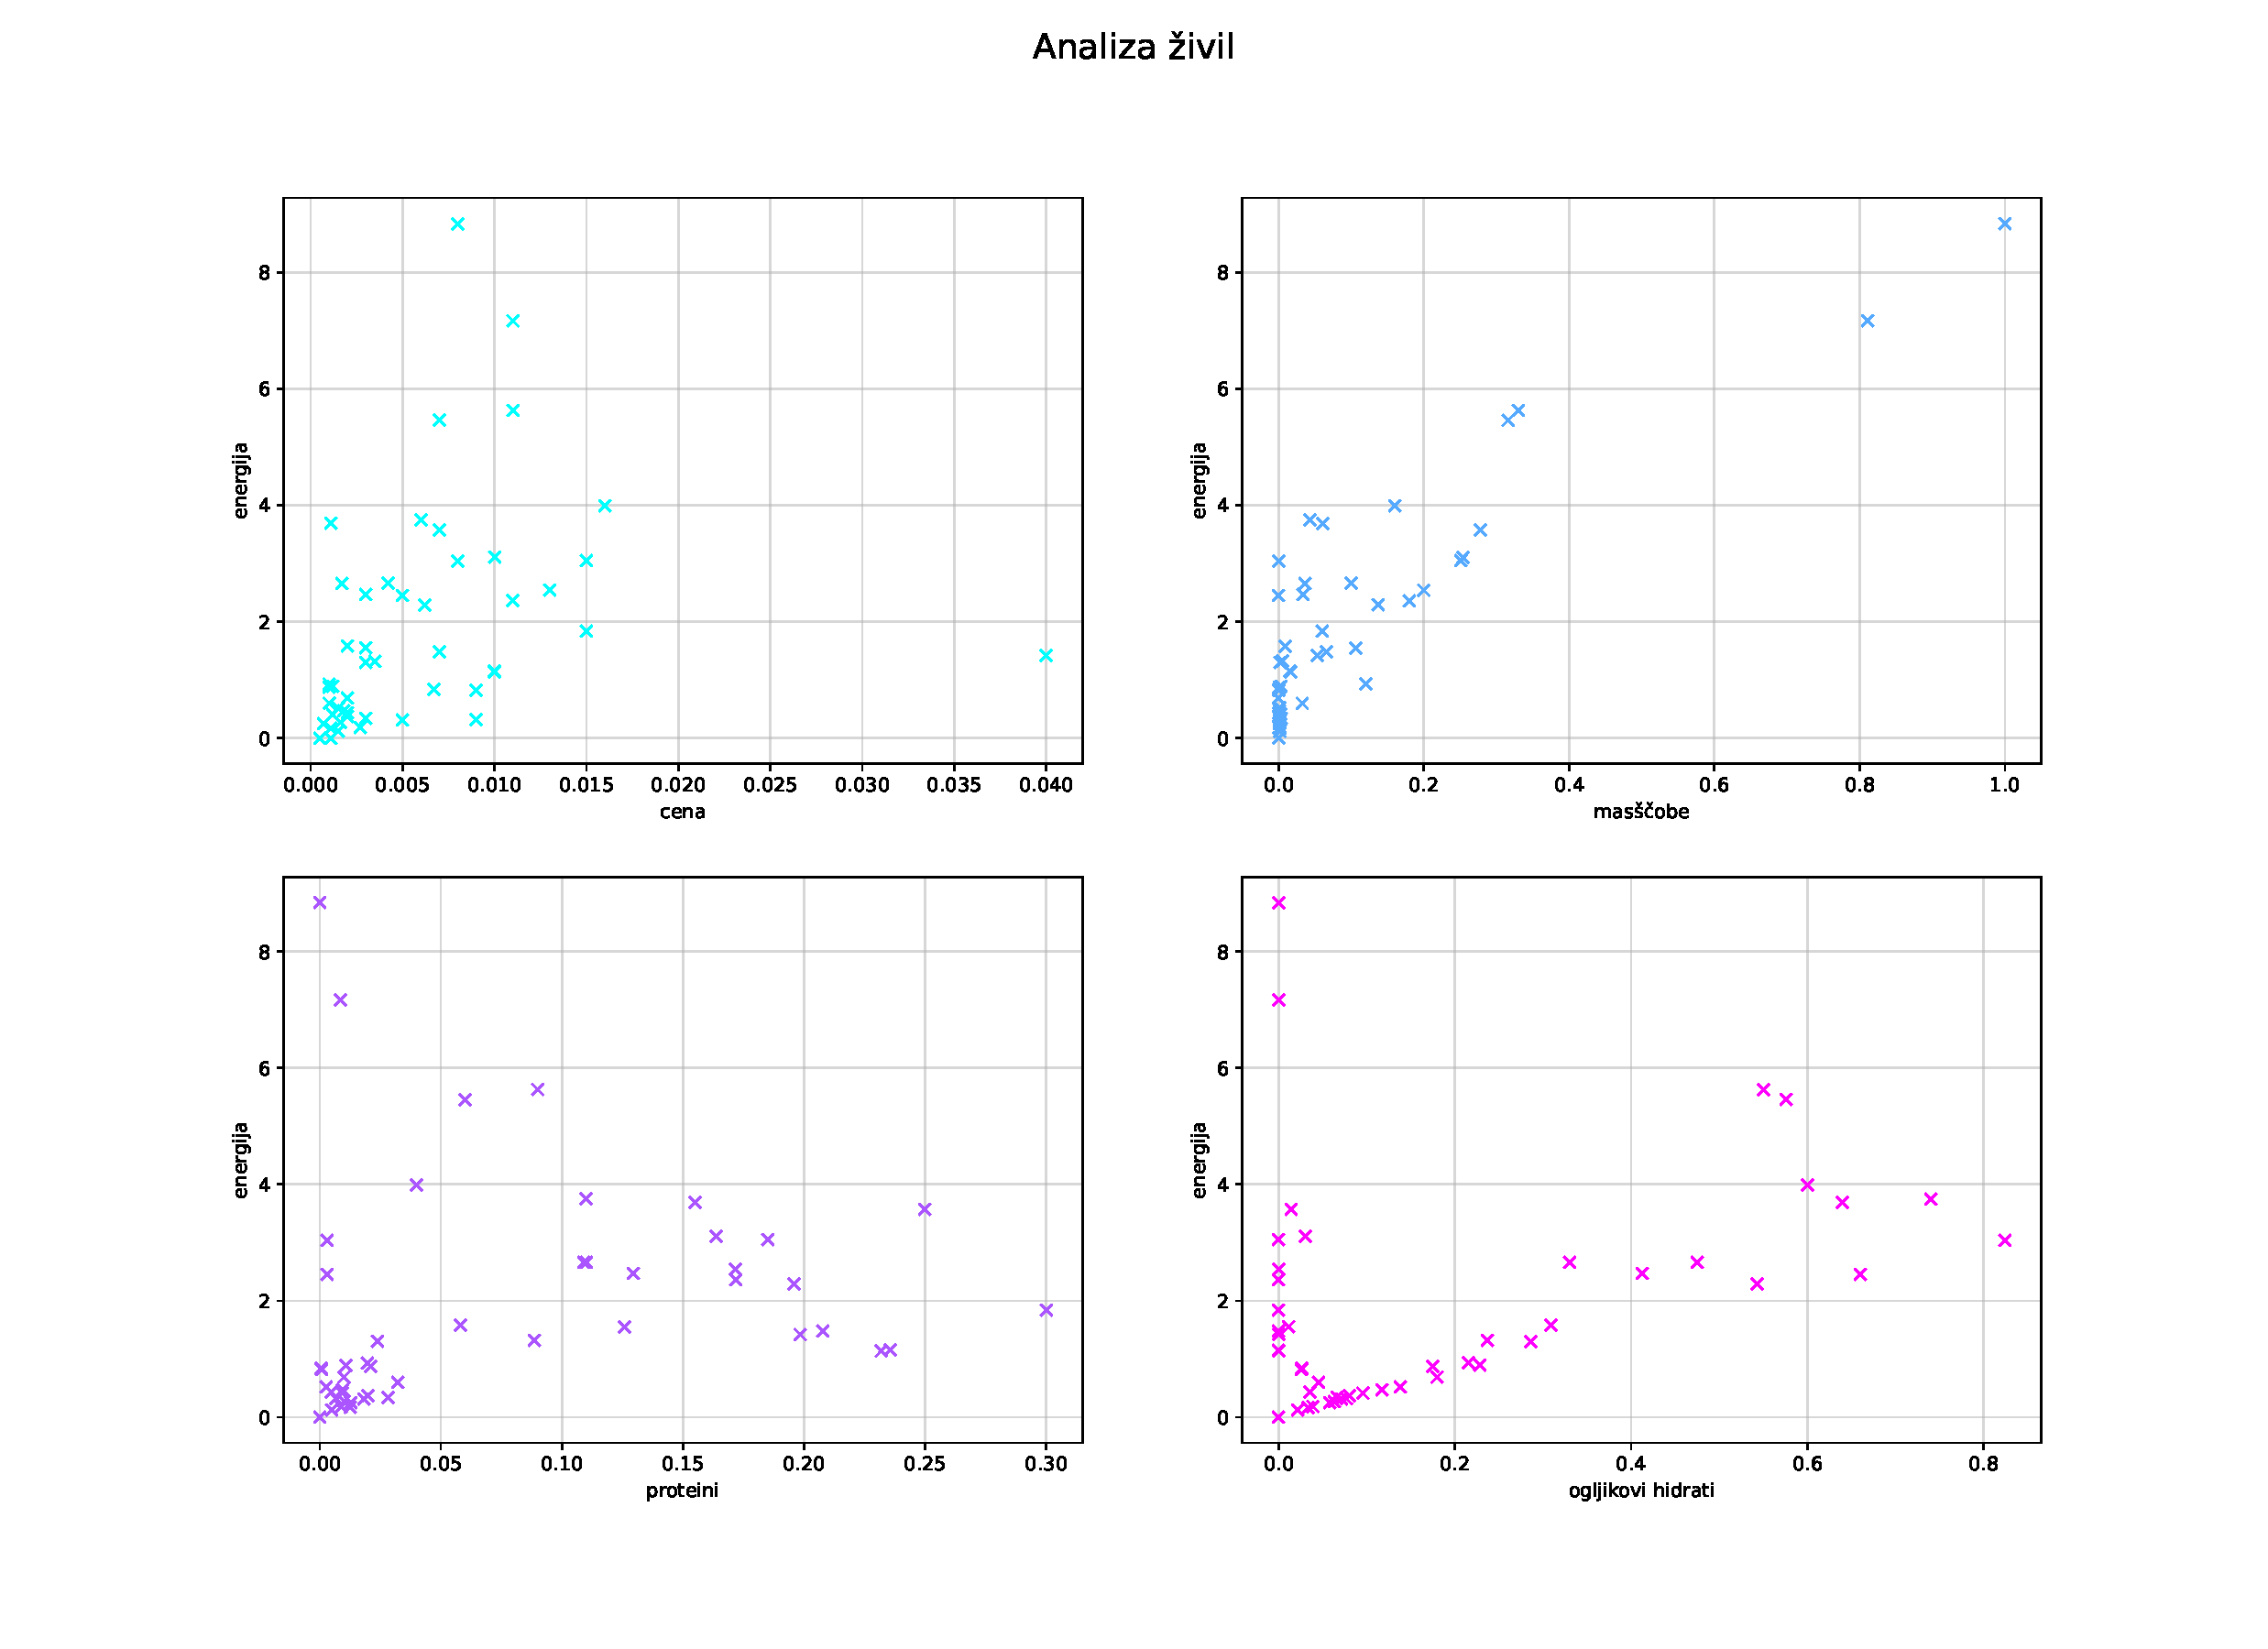
\includegraphics[width=0.95\textwidth]{grafi/analiza_zivil.pdf}
\caption{Odvisnost energijske vrednosti od cene, maščobe, proteinov in ogljikovih hidratov.}
\label{f:analiza}
\end{figure}



\section{Sestavljanje diete}
\subsection{Najmanj kalorij}
Najprej poskušamo sestavit dieto, kjer bomo zaužili najmanj kalorij, klub temu, da dosežemo dovolj vseh hranil. Prehrana je predstavljena na sliki \ref{f:lowcal}. Vidimo, da algoritem zlorablja radensko, da dobi vse minerale, ker ta pijača ne dodaja k energijski vrednosti. Tudi preostalo, kombinacija pol kilograma kakava, pomeranče in solete je za moje pojme neužitna.

\begin{figure}[H]
\centering
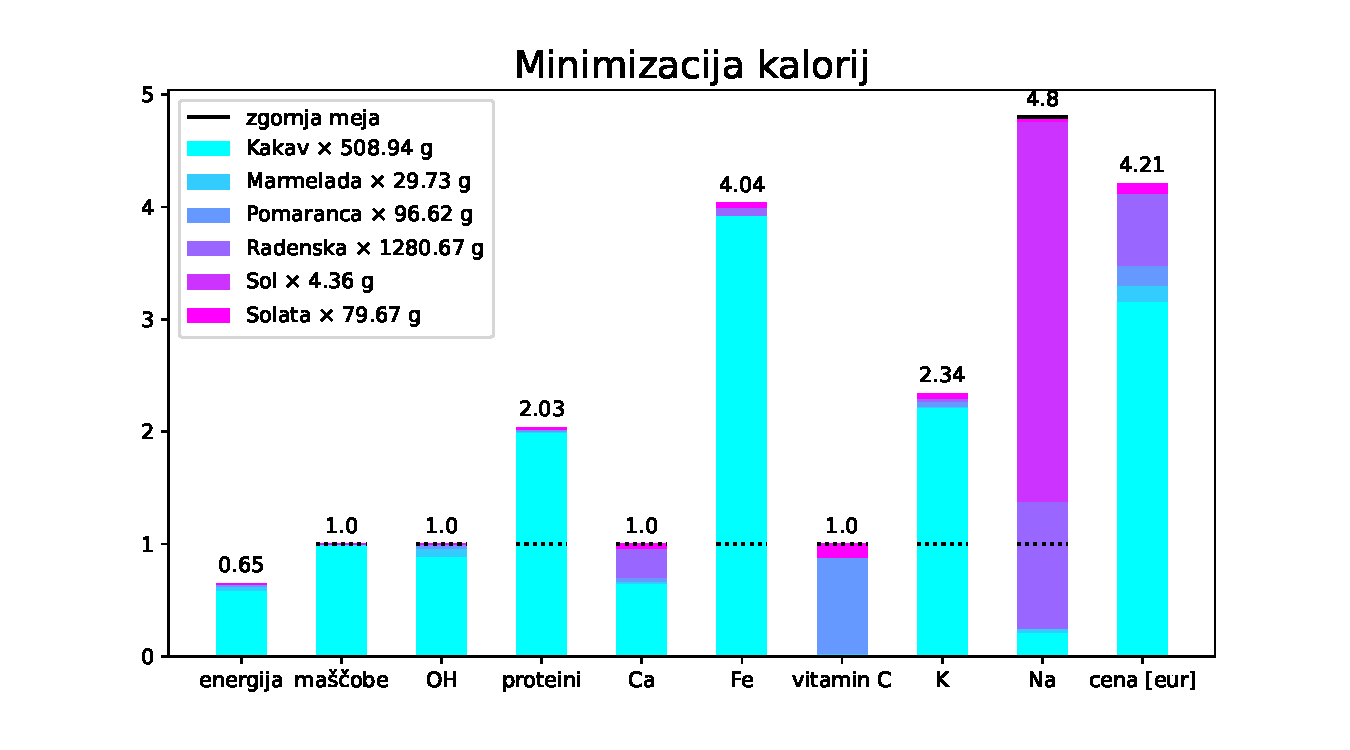
\includegraphics[width=0.85\textwidth]{grafi/graf_Low_calory_2000.pdf}
\caption{Dieta z minimalno količino kalorij. Prikaz je normiran na minimalen vnos mikroživil. Energija je normirana na 2000 kcal. Barve stoplčnega prikaza prikazujejo porazdelitev po živilih.}
\label{f:lowcal}
\end{figure}

Problem sem rešil z  omejitvijo vsakega živila na največ 300 g (slika \ref{f:lowcal_300}). Dobil sem alternativno dieto, ki doseže isto. Je bistveno bolj razgibana ampak vnesli bomo več energije in zanjo zapravili več denarja. Zanimivo je tudi to, da nismo porabili maksimalne dovoljene količine radenske. Za primer, kjer sem omejil živila na 400 g je dieta zgledala bistveno bolj podobna neomejeni.

\begin{figure}[H]
\centering
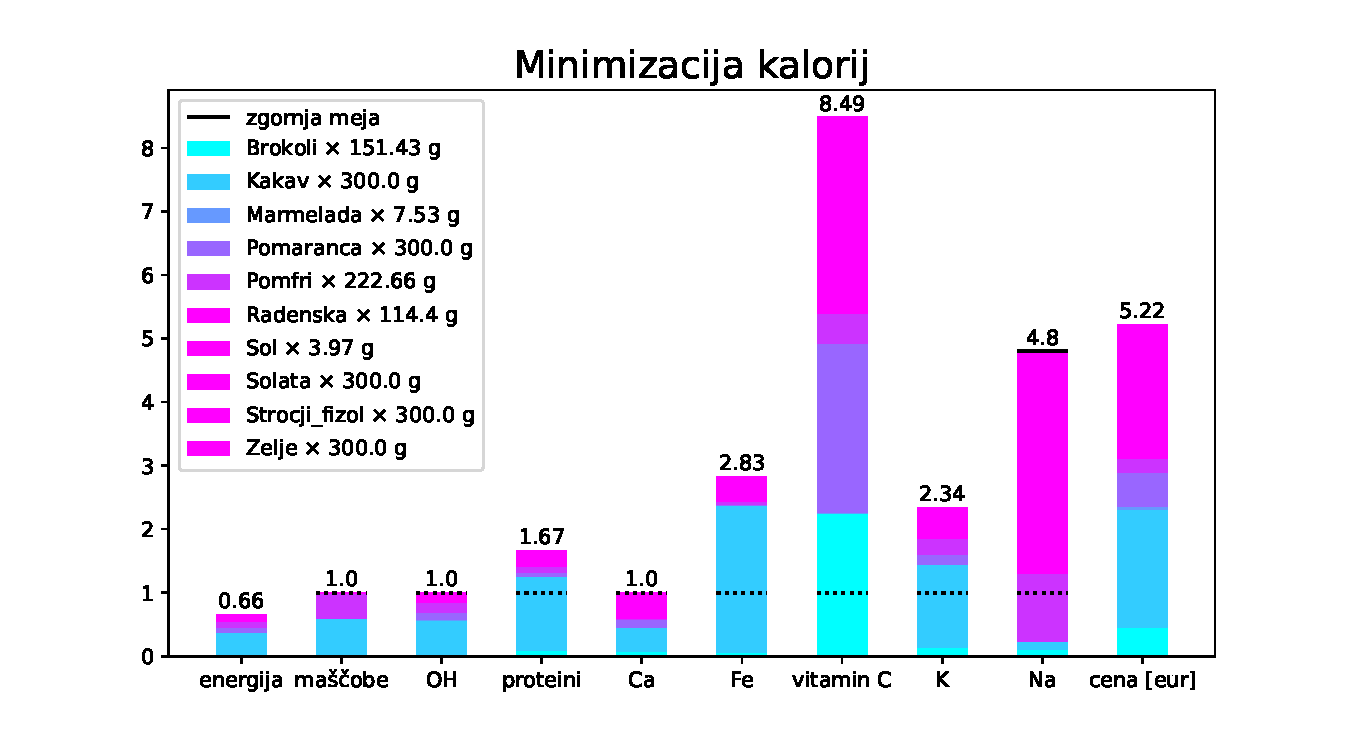
\includegraphics[width=0.85\textwidth]{grafi/graf_Low_calory_300.pdf}
\caption{Dieta z minimalno količino kalorij. Prikaz je normiran na minimalen vnos mikroživil. Energija je normirana na 2000 kcal. Barve stoplčnega prikaza prikazujejo porazdelitev po živilih. Omejitev vsakega živila na največ 300 g.}
\label{f:lowcal_300}
\end{figure}



\subsection{Najmanj maščob}
Prve diete za hujšanje so izhajale iz manjše porabe maščobe v smislu manj je poješ, manj je imaš na telesu. Pri sestavljanju take diete so rezultati popolnoma drugačni, kot pri minimizaciji vnešenih kalorij. Ponovi se le solata, ki je pa tu bistveno preveč uporabljena. Pojesti bi morali tudi pol kilograma marmelade (slika \ref{f:lowfat}).

\begin{figure}[H]
\centering
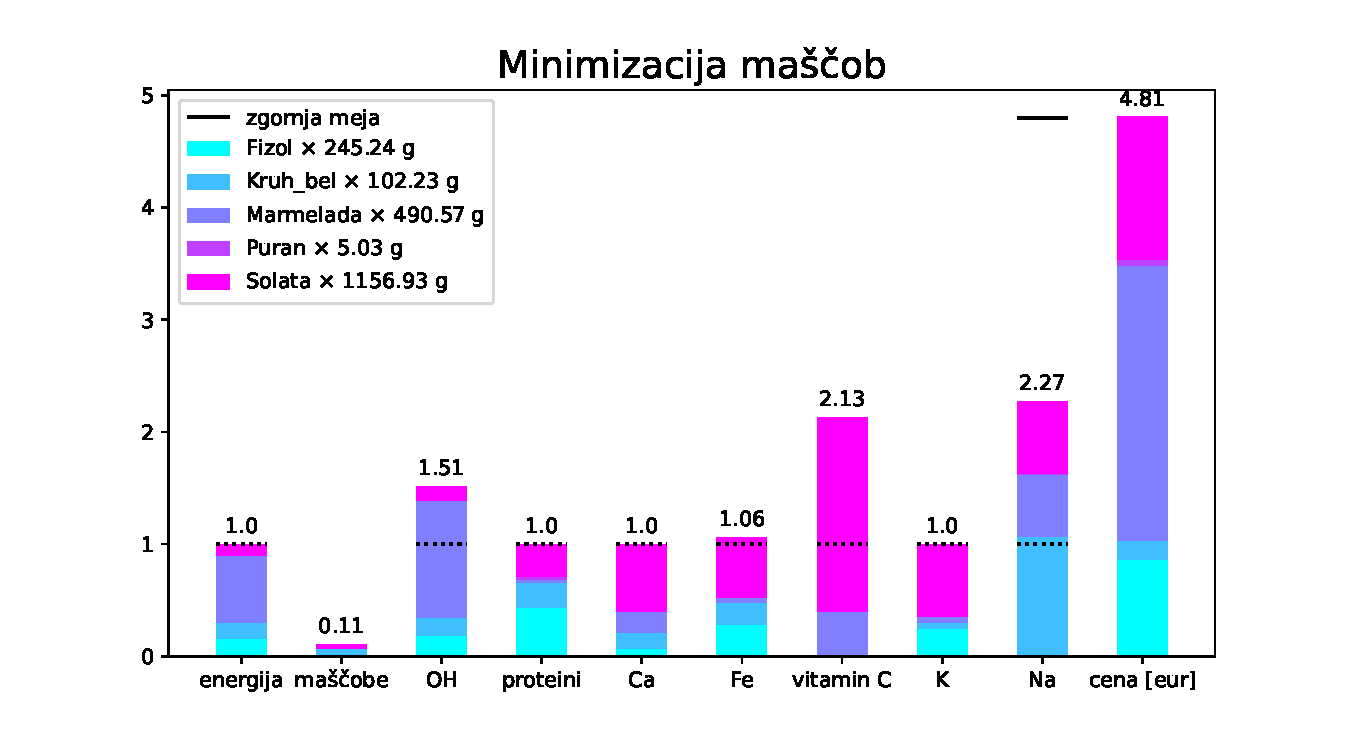
\includegraphics[width=0.85\textwidth]{grafi/graf_Low_fat_2000.pdf}
\caption{Dieta z minimalno količino maščob. Prikaz je normiran na minimalen vnos mikroživil. Maščoba je normirana na 70 g. Barve stoplčnega prikaza prikazujejo porazdelitev po živilih.}
\label{f:lowfat}
\end{figure}

Spet uporabimo isti trik kot v prejšnjem poglavju, da bo prehrana manj pusta (slika \ref{f:lowfat_300}). In spet smo nazaj pri stročjem fižolu ter zelju.

\begin{figure}[H]
\centering
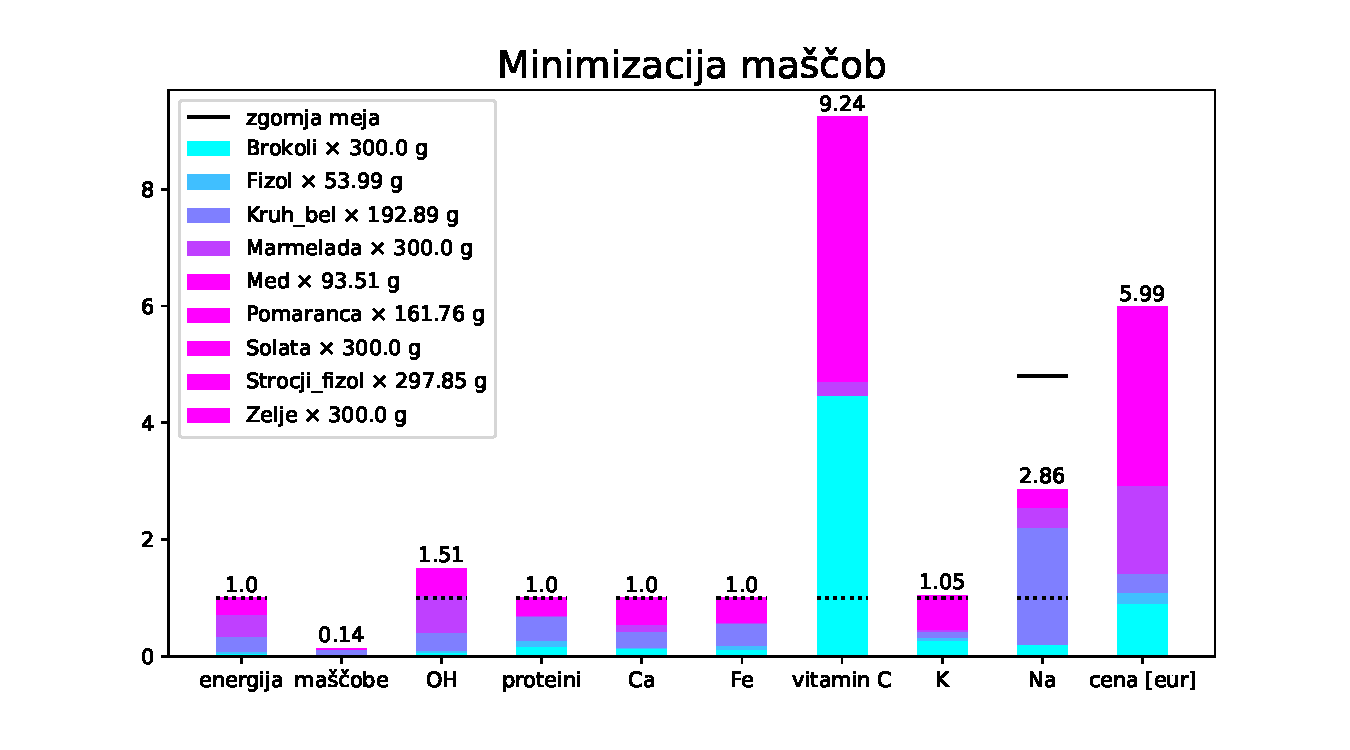
\includegraphics[width=0.85\textwidth]{grafi/graf_Low_fat_300.pdf}
\caption{Dieta z minimalno količino maščob. Prikaz je normiran na minimalen vnos mikroživil. Maščoba je normirana na 70 g. Barve stoplčnega prikaza prikazujejo porazdelitev po živilih. Omejitev vsakega živila na največ 300 g.}
\label{f:lowfat_300}
\end{figure}



\subsection{Najcenejši obrok}
Študentje na fakultetah kot je FMF zapravimo veliko časa za učenje in pisanje nalog, zato si ne moremo privoščiti redne zaposlitve in plače, ki pride z njo. Velikokrat iščemo najcenejšo prehrano ali pa vsaj tisto z najenostavnejšo pripravo. 

\begin{figure}[H]
\centering
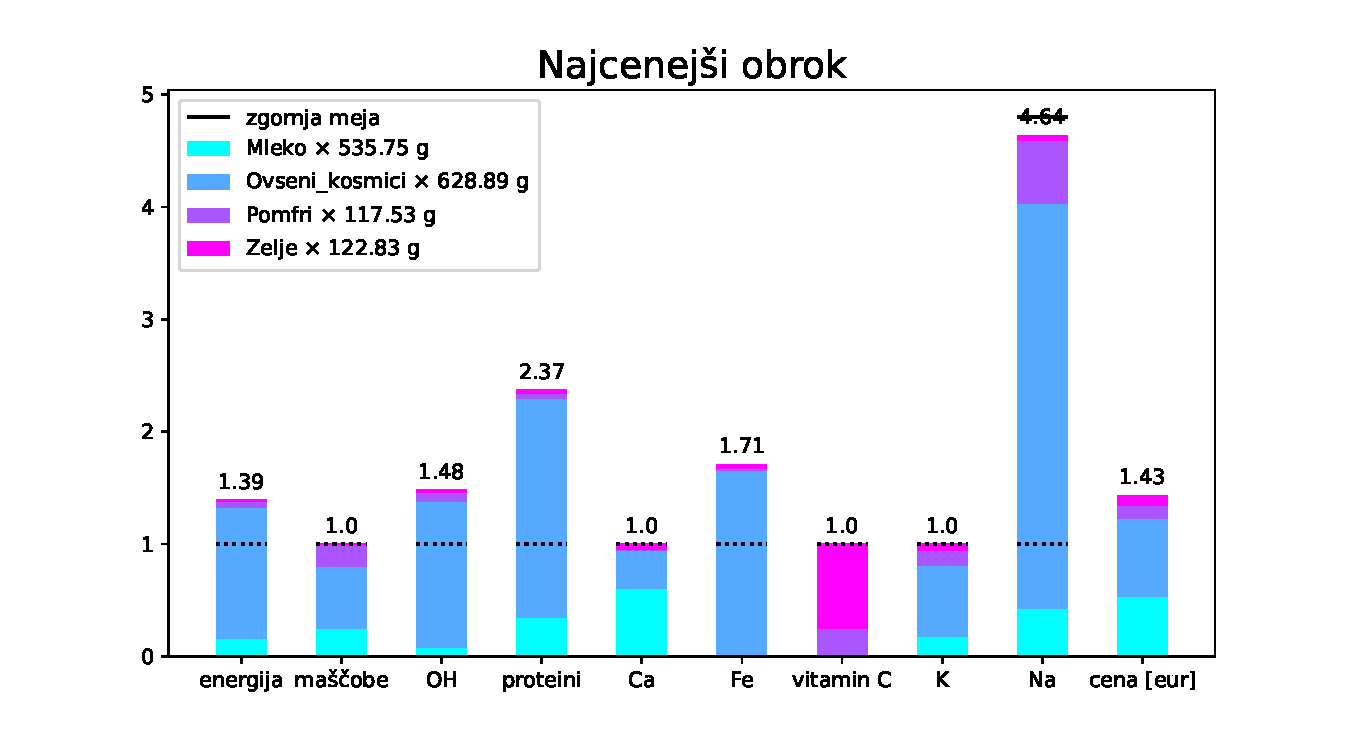
\includegraphics[width=0.85\textwidth]{grafi/graf_Low_price_2000.pdf}
\caption{Najcenejša dieta. Prikaz je normiran na minimalen vnos mikroživil. Barve stoplčnega prikaza prikazujejo porazdelitev po živilih.}
\label{f:lowprice}
\end{figure}

Slika \ref{f:lowprice} nam pove, da to lahko dosežemo s pomfritom zeljem mlekom in ovsenimi kosmiči. S temi živili lahko minimalni dnevni vnos hrane dosežemo celo za en evro manj od vrednosti študentskega bona. Omejimo zdaj vnos vsakega živila na največ 200 g. Za le 27 centov več na obrok dobimo še banano, krompir in sir. Zdaj je iz teh sestavin mogoče že sestaviti kakšno jed.

\begin{figure}[H]
\centering
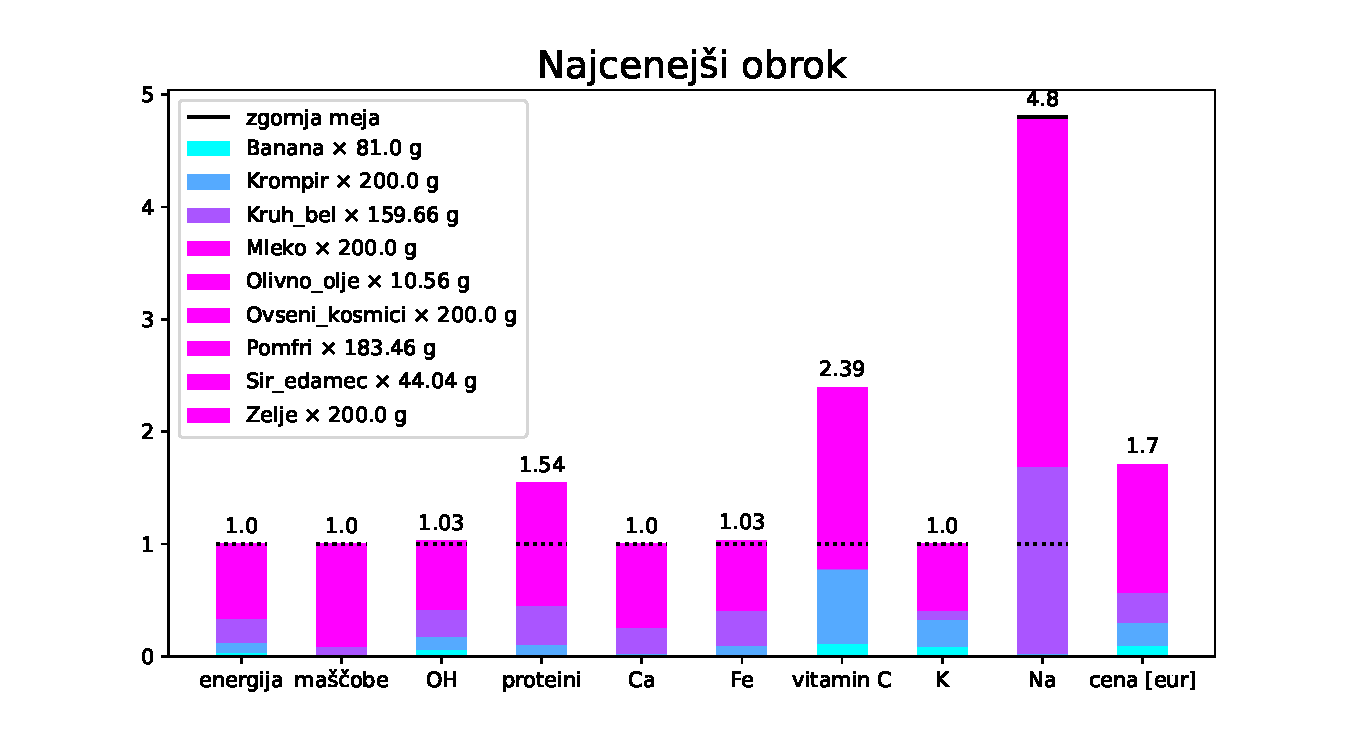
\includegraphics[width=0.85\textwidth]{grafi/graf_Low_price_200.pdf}
\caption{Najcenejša dieta. Prikaz je normiran na minimalen vnos mikroživil. Barve stoplčnega prikaza prikazujejo porazdelitev po živilih. Omejitev vsakega živila na največ 200 g.}
\label{f:lowprice_200}
\end{figure}


\subsection{LCHF dieta}
Priljubljena moderna dieta je LCHF, torej malo ogljikovih hidratov in veliko maščob. Cilj te diete je, da naučimo telo pri športu namesto OH porabljati maščobo. Tako bomo porabljali tui maščobo shranjeno v tkivih in zato hujšali. 

\begin{figure}[H]
\centering
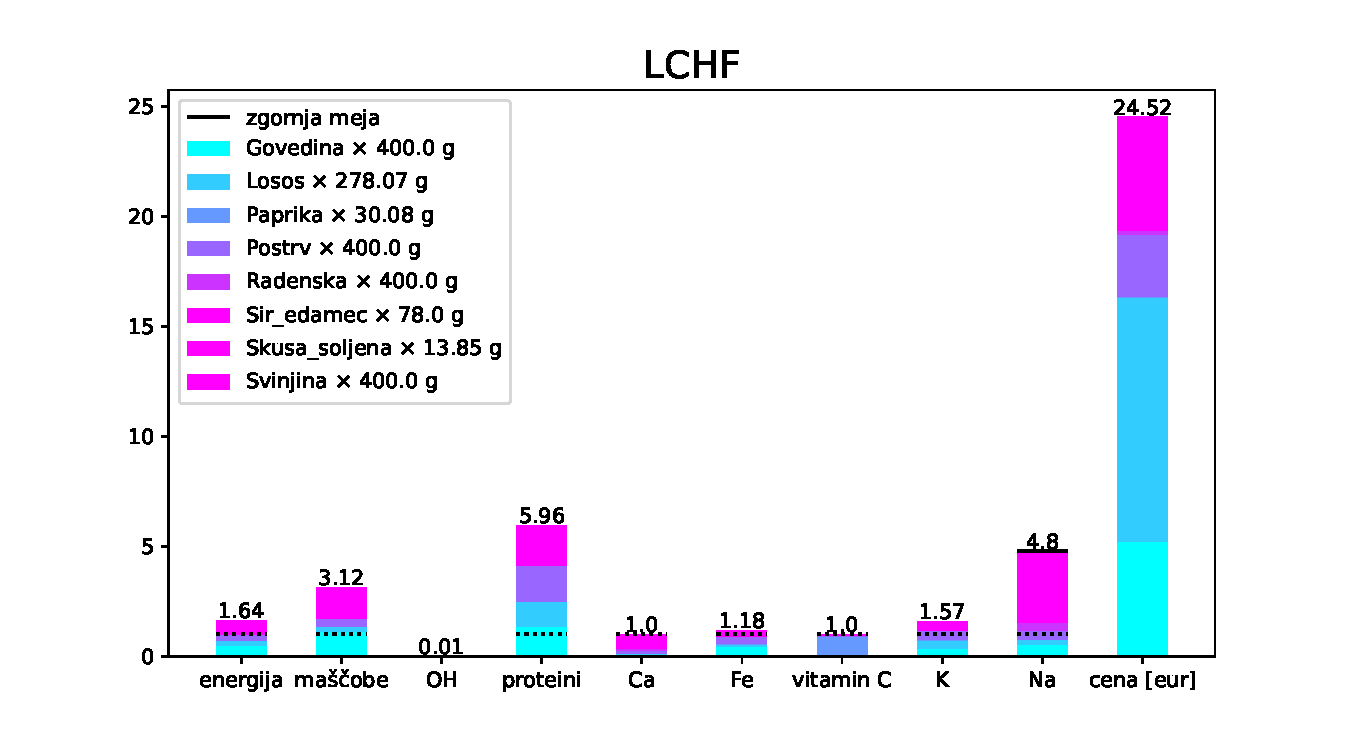
\includegraphics[width=0.85\textwidth]{grafi/graf_LCHF_400.pdf}
\caption{Dieta malo ogljikovih hidratov in veliko maščob. Prikaz je normiran na minimalen vnos mikroživil. Barve stoplčnega prikaza prikazujejo porazdelitev po živilih. Omejitev vsakega živila na največ 400 g.}
\label{f:LCHF_400}
\end{figure}

Na sliki \ref{f:LCHF_400} vidimo, da energijo, ki bi jo dobili iz ogljikovih hidratov nadomestimo z maščobami in proteini, katerih pojemo trikratno in petkratno vrednost. Pojemo veliko rdečega mesa in ribe, zato tudi cena občutno naraste. Spet minerale dobimo iz maksimalne količine radenske.


\end{document}